\documentclass{beamer}


%%%%%%%%%%%%%%%%%%%%%%%%%%%%%%%%%%%%%%%%%%%%%%%%%%%%
% THEME
%
% For more themes, color themes and font themes, see:
% http://deic.uab.es/~iblanes/beamer_gallery/index_by_theme.html

\mode<presentation>
{
  \usetheme{Madrid}   % or try Darmstadt, Copenhagen, Madrid, Warsaw, Berlin, ...
  \usecolortheme{beaver} % or try albatross, beaver, crane, rose, ...
  \usefonttheme{serif}  % or try serif, structurebold, ...
  \setbeamertemplate{navigation symbols}{%
    %\insertframenavigationsymbol
    %\insertsubsectionnavigationsymbol
    \insertsectionnavigationsymbol}
  \setbeamertemplate{caption}[numbered]
}

% Berlin theme's footer + page number
\makeatletter
  \setbeamertemplate{footline}{%
    \begin{beamercolorbox}[colsep=1.5pt]{upper separation line foot}
    \end{beamercolorbox}
    \begin{beamercolorbox}[ht=2.5ex,dp=1.125ex,%
      leftskip=.3cm,rightskip=.3cm plus1fil]{author in head/foot}%
      \leavevmode{\usebeamerfont{author in head/foot}\insertshortauthor}%
      \hfill%
      {\usebeamerfont{institute in head/foot}\usebeamercolor[fg]{institute in head/foot}\insertshortinstitute}%
    \end{beamercolorbox}%
    \begin{beamercolorbox}[ht=2.5ex,dp=1.125ex,%
      leftskip=.3cm,rightskip=.3cm plus1fil]{title in head/foot}%
      {\usebeamerfont{title in head/foot}\insertshorttitle\hfill\insertframenumber/\inserttotalframenumber}%
    \end{beamercolorbox}%
    \begin{beamercolorbox}[colsep=1.5pt]{lower separation line foot}
    \end{beamercolorbox}
  }
\makeatletter


% For backup slide fooling page counter
%\usepackage{beamerthemesplit}
\newcommand{\backupbegin}{
   \newcounter{finalframe}
   \setcounter{finalframe}{\value{framenumber}}
}
\newcommand{\backupend}{
   \setcounter{framenumber}{\value{finalframe}}
}





%%%%%%%%%%%%%%%%%%%%%%%%%%%%%%%%%%%%%%%%%%%%%%%%%%%%
% PACKAGES

\usepackage[english]{babel}
\usepackage[utf8x]{inputenc}
\usepackage{enumitem}

\usepackage{graphicx}
%\usepackage{subfloat}
\usepackage{subfig}

\usepackage{xcolor}
    \definecolor{myred}{RGB}{127, 0, 0}
    \definecolor{myyellow}{RGB}{127, 106, 0}

\usepackage{minted} % Display code
    \usemintedstyle{tango}
    
\usepackage{lipsum}





%%%%%%%%%%%%%%%%%%%%%%%%%%%%%%%%%%%%%%%%%%%%%%%%%%%%
% COMMANDS
\AtBeginSection[]
{
  \begin{frame}<beamer>
    \frametitle{Plan}
    \tableofcontents[currentsection,currentsubsection]
  \end{frame}
}

\let\oldfootnotesize\footnotesize
\renewcommand*{\footnotesize}{\oldfootnotesize\tiny}

\def\includeBlockDiagram{1}
\if\includeBlockDiagram1
    \usepackage{tikz}
    \usetikzlibrary{shapes,arrows}
    \usepackage{verbatim}
    \usetikzlibrary{positioning}
    \usepackage{bm}
\fi

\newcommand{\TODO}[1]{{\color{red}\textbf{TODO} #1}}





%%%%%%%%%%%%%%%%%%%%%%%%%%%%%%%%%%%%%%%%%%%%%%%%%%%%
% TITLE
\title[Deep Learning-based Speech Enhancement]{Deep Learning-based Speech Enhancement}
\author{Paul \textsc{Aimé}, \\ Antoine \textsc{Bertrand}}
\institute{3A SICOM EEH}
\date{\today}





%%%%%%%%%%%%%%%%%%%%%%%%%%%%%%%%%%%%%%%%%%%%%%%%%%%%
% DOCUMENT

\begin{document}

\begin{frame}
  \titlepage
\end{frame}










% ==================================================
\section{Jeu de données}


\begin{frame}{Jeu de parole}

\begin{itemize}[label=$\bullet$]
    \item \textit{TIMIT Speech Corpus}~\cite{abdelaziz2017timit}.
    \item 630 locuteurs des huit dialectes majeurs de l'anglais américain,
    \item Lecture de phrases phonétiquement riches de $\sim$ 3 secondes.
    \item Ratio d'entraînement (train - val) = (87,8\% - 12,2\%)
\end{itemize}

\begin{table}[!h]
\center
%\resizebox{\textwidth}{!}{%
\begin{tabular}{ |c|c|c|c| } 
\hline
    & Train Set & Validation Set & Test Set \\ 
    \hline
    Nombre & 4056 & 564 & 1680 \\ 
    \hline
    Pourcentage & 64,4\% & 9,0\% & 26,6\% \\
    \hline
\end{tabular}%
%}
    \captionsetup{justification=centering,margin=2cm}
    \caption{Répartition des enregistrements de parole dans les différents jeux de données.}
    \label{tab:nb_sounds_per_database}
\end{table}

\end{frame}




\begin{frame}{Jeu de bruit}
\begin{itemize}[label=$\bullet$]
    \item Fichier .wav de 3min30
    \item Bruit d'ambiance de voix humaines
    \item Ratio d'entraînement (train - val) = (87,8\% - 12,2\%)
\end{itemize}

\begin{table}[]
\center
\resizebox{\textwidth}{!}{%
\begin{tabular}{ |c|c|c|c| } 
    \hline
    & babble\_train.wav & babble\_val.wav & babble\_test.wav \\ 
    \hline
    Tronçon & 0:00 - 3:00 & 3:00 - 3:25 & 3:25 - 3:55 \\ 
    \hline
    Durée & 180s & 25s & 30s \\ 
    \hline
    Pourcentage & 76,6\% & 10,6\% & 12,8\% \\
    \hline
\end{tabular}%
}
\captionsetup{justification=centering,margin=0cm}
\caption{Découpage du fichier de bruit.}
\label{tab:dataset_repartition}
\end{table}
\end{frame}




\begin{frame}{Mixage}
\begin{figure}
    \centering
    \resizebox{\linewidth}{!}{%
        \input{block_diagrams/mixage.tex}
    }
    \captionsetup{justification=centering,margin=1cm}
    \caption{Schéma bloc de la fonction de mixage \texttt{add\_noise\_snr(signal, noise, snr\_dB)}}
    \label{fig:block_mixage}
\end{figure}
\end{frame}




\begin{frame}[fragile]{STFT}
\begin{columns}
    \begin{column}{0.5\textwidth}
        \scriptsize{%
        \begin{description}[align=right, leftmargin=*, labelindent=2.5cm]
            \item[fréquence :] 8 kHz
            \item[nfft :] 256 (32 ms)
            \item[overlap :] 50\%
        \end{description}}
    \end{column}%
    \hfill%
    \begin{column}{0.5\textwidth}
        \scriptsize{%
        \begin{description}[align=right, leftmargin=*, labelindent=2.5cm]
            \item[apodisation :] hanning
            \item[centrage :] oui
            \item[padding :] réflection
        \end{description}}
    \end{column}%
\end{columns}
\begin{figure}[]
    \centering
    \subfloat[][Clean]{%
        \includegraphics[width=.45\linewidth]{imgs/SA2_clean.png}
    }
    \hfill%
    \subfloat[][Noisy]{%
        \includegraphics[width=.45\linewidth]{imgs/SA2_noisy.png}
    }
    \captionsetup{justification=centering,margin=0cm}
    \caption{Exemples de STFTs de signal d'origine et de signal bruité.}
    \label{fig:loss_plot}
\end{figure}
\end{frame}










% ==================================================
\section{Modèle}

\begin{frame}{Encodeur-Décodeur Convolutionnel}
\begin{figure}[H]
    \centering
    \includegraphics[width=.6\linewidth]{imgs/redundant_enco_deco.png}
    \captionsetup{justification=centering,margin=0cm}
    \caption{Architecture du réseau R-CED proposé dans~\cite{park2017}. \\ \tiny{Figure issue de l'article correspondant.}}
    \label{fig:RCED_architecture}
\end{figure}
\end{frame}




\begin{frame}{Paramètres d’architecture}

\begin{description}[align=right, leftmargin=*, labelindent=4cm]
    \item[Entrée :] $(H, W) = (129, 7)$ 
    \item[Durée :] $32 + 6 \times 16 = 128$ ms\footnotemark
    \item[Nb paramètres :] $32611$ 
\end{description}

\begin{table}[]
\resizebox{\textwidth}{!}{%
\begin{tabular}{|r|c|c|c|c|c|c|c|c|c|c|}
\hline
\multicolumn{1}{|l|}{}              & \multicolumn{4}{c|}{\textbf{Encoder}}      & \textbf{Latent} & \multicolumn{4}{c|}{\textbf{Decoder}}     & \textbf{Out} \\ \hline
\textbf{Layer}                      & 1         & 2        & 3        & 4        & 5               & 6        & 7        & 8        & 9        & 10           \\ \hline
\textbf{(in, out)} & (1, 12)   & (12, 16) & (16, 20) & (20, 24) & (24, 32)        & (32, 24) & (24, 20) & (20, 16) & (16, 12) & (12, 1)     \\ \hline
\textbf{kernel size}                & (13, $W$=7) & (11, 1)  & (9, 1)   & (7, 1)   & (7, 1)          & (7, 1)   & (9, 1)   & (11, 1)  & (13, 1)  & ($H$=129, 1)   \\ \hline
\end{tabular}}
\captionsetup{justification=centering,margin=0cm}
\caption{Paramètres de \textit{feature maps} et de taille du noyau de convolution pour chaque couche du modèle.}
\label{tab:layers_params}
\end{table}
\footnotetext{\cite{park2017} utilise 88ms.}
\end{frame}




\begin{frame}{Construction du batch}
\begin{description}[align=right, leftmargin=*, labelindent=4.5cm]
    \item[Entrée :] $(H, W) = (129, 7)$
    \item[Taille du batch :] un fichier son
    \item[Saut entre les entrées :] 1
    \item[Entrées par batch :] $N$, le nombre de frame de la STFT du son (3s $\rightarrow$ 187)
    \item[~]
    \item[Sortie :] $(N, H, 1) \longrightarrow (N, H)$
\end{description}
\end{frame}










% ==================================================
\section{Apprentissage}


\begin{frame}{Procédure}
\begin{figure}
    \centering
    \resizebox{\linewidth}{!}{%
        \input{block_diagrams/training.tex}
    }
    \captionsetup{justification=centering,margin=0cm}
    \caption{Schéma bloc de la procédure d'apprentissage.}
    \label{fig:block_training}
\end{figure}
\end{frame}




\begin{frame}{Évaluation de l’apprentissage}

\only<2>{{\scriptsize
\begin{description}
    \item[Librairie :] PyTorch~\cite{pytorch}.
    \item[Machine :] GCP Compute Engine \texttt{n1-highmem-8}
    \item[Puissance :] 8 vCPU et 1 GPU NVIDIA Tesla P4.
    \item[Durée d'une époque :] 6 min 15 + 15 sec (50 époques = 6 heures)
\end{description}}

\vspace{-10pt}}

\begin{figure}[]
    \centering
    \subfloat[][$RSB=0 dB$]{%
        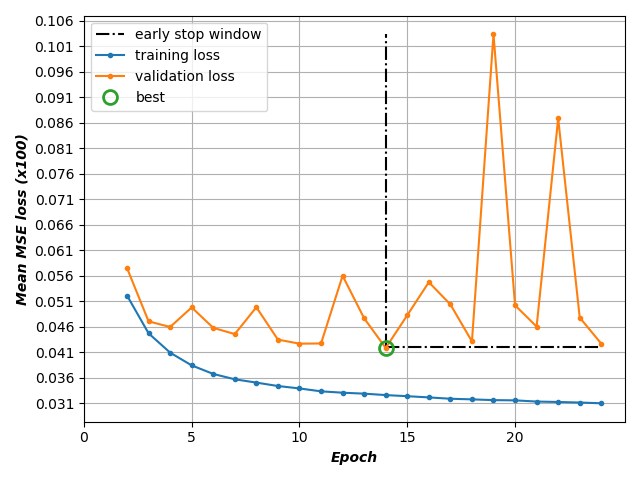
\includegraphics[width=.3\linewidth]{imgs/loss_plot/fs8000_snr0_nfft256_hop128.png}
    }
    \hfill%
    \subfloat[][$RSB=-5 dB$]{%
        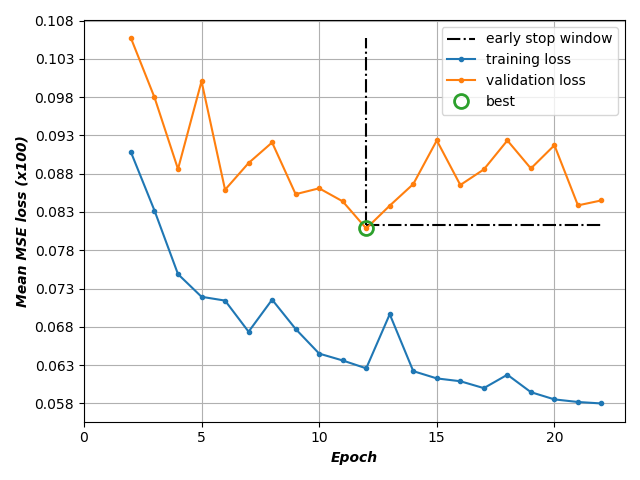
\includegraphics[width=.3\linewidth]{imgs/loss_plot/fs8000_snr-5_nfft256_hop128.png}
    }
    \hfill%
    \subfloat[][$RSB=-20 dB$]{%
        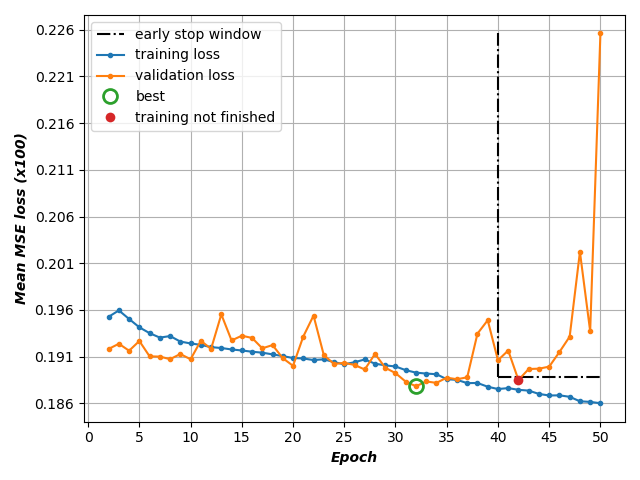
\includegraphics[width=.3\linewidth]{imgs/loss_plot/fs8000_snr-20_nfft256_hop128.png}
    }
    \captionsetup{justification=centering,margin=0cm}
    \caption{Évolution des erreurs quadratiques moyennes (EQM) d’entraînement, pour des modèles entraînés sur des jeux de données à différents niveau de RSB. La première époque n'est pas représentée.}
    \label{fig:loss_plot}
\end{figure}
\end{frame}










% ==================================================
\section{Prédiction}


\begin{frame}{Procédure}
\begin{figure}
    \centering
    \resizebox{\linewidth}{!}{%
        \input{block_diagrams/prediction.tex}
    }
    \captionsetup{justification=centering,margin=0cm}
    \caption{Schéma bloc de la procédure de débruitage.}
    \label{fig:block_prediction}
\end{figure}
\end{frame}



\begin{frame}{Reconstruction du signal audio}
\begin{itemize}
    \item RSB \textbf{sans} étape de normalisation:  140.33 dB
    \item RSB \textbf{avec} étape de normalisation:  2.76 dB
\end{itemize}

\begin{figure}
    \centering
    \resizebox{\linewidth}{!}{%
        \input{block_diagrams/reconstruction_pblm.tex}
    }
    \captionsetup{justification=centering,margin=0cm}
    \caption{Schéma bloc d'une procédure de reconstruction simple.}
    \label{fig:block_probleme_reocnstruction}
\end{figure}
\end{frame}










% ==================================================
\section{\'Evaluation / Résultats}

\begin{frame}{\'Evaluation par comparaison des spectrogrammes}
\only<1>{%
\begin{figure}[H]
    \centering
    \includegraphics[width=.7\linewidth]{imgs/eval/SA2_clean.png}
    \captionsetup{justification=centering,margin=0cm}
    \caption{STFT du signal d'origine non bruité}
    \label{fig:STFTbruite}
\end{figure}%
}

\only<2>{%
\begin{figure}[H]
    \centering
    \includegraphics[width=.7\linewidth]{imgs/eval/SA2_noisy.png}
    \captionsetup{justification=centering,margin=0cm}
    \caption{STFT du signal bruité}
    \label{fig:STFTbruite}
\end{figure}
}

\only<3>{%
\begin{figure}[H]
    \centering
    \includegraphics[width=.7\linewidth]{imgs/eval/SA2_pred.png}
    \captionsetup{justification=centering,margin=0cm}
    \caption{STFT débruitée prédite}
    \label{fig:STFTbruite}
\end{figure}
}

\only<4>{%
\begin{figure}[]
    \centering
    \subfloat[][STFT du signal bruité]{%
        \includegraphics[width=.32\linewidth]{imgs/eval/SA2_noisy.png}
    }
    \hfill%
    \subfloat[][STFT débruitée prédite]{%
        \includegraphics[width=.32\linewidth]{imgs/eval/SA2_pred.png}
    }
    \hfill%
    \subfloat[][STFT du signal d'origine non bruité]{%
        \includegraphics[width=.32\linewidth]{imgs/eval/SA2_clean.png}
    }
    \captionsetup{justification=centering,margin=1cm}
    \caption{Visualisation des spectrogrammes d'un signal avant, pendant, et après débruitage. \\(SNR d'entrée = 0dB)}
    \label{fig:stfts}
\end{figure}
}
\end{frame}

\begin{frame}{\'Evaluation par comparaison des spectrogrammes}
\begin{figure}[H]
    \centering
    \includegraphics[width=.7\linewidth]{imgs/eval/diff3.png}
    \captionsetup{justification=centering,margin=0cm}
    \caption{Visualisation des différences entre les spectrogrammes du signal non bruité et le spectrogramme débruité prédit.\\}
    \label{fig:diff}
\end{figure}
\end{frame}


\begin{frame}{\'Evaluation du gain en RSB}
\begin{figure}
    \centering
    \resizebox{.7\linewidth}{!}{%
        \input{block_diagrams/evaluation.tex}}
    
    \captionsetup{justification=centering,margin=0cm}
    \caption{Schéma bloc de la procédure d'évaluation.}
    \label{fig:block_evaluation}
\end{figure}
\begin{table}[!h]
\begin{center}
\scalebox{0.7}{
\begin{tabular}{ |c||c|c|c|c|  }
 \hline
 \textbf{Input SNR (clean vs noisy)} & \textbf{-20dB} & \textbf{-10dB} & \textbf{-5dB} & \textbf{0dB}\\ 
 \hline
 Mean SNR (clean vs pred) & 1.859163 & 1.859163 & 1.859163 & 1.859163\\ 
 \hline
 STD SNR (clean vs pred) & 0.734523 & 0.734523 & 0.734523 & 0.734523\\ 

\hline
\end{tabular}}
\end{center}
    \RawCaption{\caption{Statistiques calculées sur les valeurs de SNR des sons du jeu de test.}
    \label{tab:snr_stats}}
\end{table}
\end{frame}


\begin{frame}{\'Evaluation subjective par écoute }
\begin{figure}[]
\centering
    \includegraphics[width=.4\linewidth]{imgs/eval/listening.png}
    \captionsetup{justification=centering,margin=0cm}
    \label{fig:listen}
\end{figure}
\end{frame}

\begin{frame}{}
  \centering \Huge
  \emph{Fin}
\end{frame}





% ==================================================
% References
\begin{frame}[allowframebreaks]
\frametitle{References}
\bibliographystyle{apalike}
\footnotesize{
    \bibliography{refs.bib}
}
\end{frame}




% ==================================================
% References

\appendix
\backupbegin

\begin{frame}{Annexe 1: Spectrogrammes prédits pour différents RSB d'entrée}
\begin{figure}[]
    \centering
    \subfloat[][SNR  d'entrée = -20dB]{%
        \includegraphics[width=.32\linewidth]{imgs/eval/SA2_pred_-20.png}
    }
    \hfill%
    \subfloat[][SNR  d'entrée = -5dB]{%
        \includegraphics[width=.32\linewidth]{imgs/eval/SA2_pred_-5.png}
    }
    \hfill%
    \subfloat[][SNR  d'entrée = 0dB]{%
        \includegraphics[width=.32\linewidth]{imgs/eval/SA2_pred.png}
    }
    \captionsetup{justification=centering,margin=1cm}
    \caption{Spectrogrammes d’un même signal débruité, avec des niveaux de bruit différents}
    \label{fig:stfts}
\end{figure}
\end{frame}


\begin{frame}{Annexe 2: Différentes architectures}
\begin{figure}[]
    \centering
    \subfloat[][]{%
        \includegraphics[width=.32\linewidth]{imgs/simple_cnn.png}
    }
    \hfill%
    \subfloat[][]{%
        \includegraphics[width=.32\linewidth]{imgs/encoder_decoder.png}
    }
    \hfill%
    \subfloat[][]{%
        \includegraphics[width=.32\linewidth]{imgs/redundant_enco_deco.png}
    }
    \captionsetup{justification=centering,margin=1cm}
    \caption{Différentes architectures}
    \label{fig:stfts}
\end{figure}
\end{frame}

\backupend


\end{document}
